\documentclass[11pt,a4paper]{article}
\usepackage[T1]{fontenc}
\usepackage[utf8]{inputenc}
\usepackage{lmodern,microtype,amsmath,amssymb,graphicx,booktabs,array,longtable,caption,geometry,titlesec,xcolor}
\usepackage[numbers,sort&compress]{natbib}
\usepackage[colorlinks=true,linkcolor=blue!50!black,citecolor=blue!50!black,urlcolor=blue!50!black]{hyperref}
\geometry{left=2.5cm,right=2.5cm,top=1.8cm,bottom=2.5cm}
\captionsetup{font=footnotesize,labelfont=bf,skip=3pt}
\titleformat{\section}{\normalfont\large\bfseries}{\thesection}{.6em}{}
\titleformat{\subsection}{\normalfont\normalsize\bfseries}{\thesubsection}{.6em}{}
\titlespacing*{\section}{0pt}{1.3ex plus .2ex minus .1ex}{.65ex}
\titlespacing*{\subsection}{0pt}{.9ex plus .1ex}{.4ex}
\setlength{\parindent}{1em}
\setlength{\parskip}{0pt}
\setlength{\textfloatsep}{7pt plus 1pt minus 1pt}
\setlength{\floatsep}{6pt plus 1pt minus 1pt}
\setlength{\intextsep}{6pt plus 1pt minus 1pt}
\setlength{\abovedisplayskip}{5pt plus 1pt minus 1pt}
\setlength{\belowdisplayskip}{5pt plus 1pt minus 1pt}
\renewcommand{\topfraction}{.95}
\renewcommand{\bottomfraction}{.95}
\renewcommand{\textfraction}{.05}
\renewcommand{\floatpagefraction}{.8}
\setcounter{topnumber}{3}
\setcounter{bottomnumber}{3}
\setcounter{totalnumber}{5}
\newcommand{\arcsinh}{\operatorname{asinh}}
\newcommand{\relu}{\operatorname{ReLU}}
\newcommand{\supp}[1]{Supplement~#1}
\graphicspath{{figures/}{figures/supplement/}}

\begin{document}
\begin{center}
{\Large\bfseries Benchmarking Comparative Single-Cell Analysis\\of CMV Status\par}
\vspace{3pt}
Sebastian Fay \quad Marie Schygulla \quad Gregor Habitzreither
\end{center}
\vspace{-6pt}

\section{Introduction}
A clinical label describes a donor, whereas the informative signal may occur in only a small subset of that donor's cells. CellCNN addresses this mismatch through supervised representation learning: shared cell filters and pooling are trained jointly to predict a sample-level outcome, allowing rare, informative responses to influence the representation~\cite{cellcnn}. This differs from first clustering cells and classifying their population frequencies, as in Citrus~\cite{citrus}, or labelling every training cell with its donor's outcome, as in a single-cell SVM. The paper also compares logistic regression, random forests, distance-based outlier detection, single-marker gates, moment summaries and a denoising autoencoder. \supp{S1} distinguishes these literature baselines from our implemented methods. Moment summaries and autoencoders describe samples before outcome prediction, while outlier detection and marker gates identify candidate cells through distance or expression thresholds. Sample classification and recovery of an informative cell subset therefore require separate evaluation.

We study the supplied CMV cohort derived from Horowitz et al.~\cite{horowitz}. CMV exposure is associated with expansions of NKG2C/CD57-expressing NK populations, but neither donor status nor a marker average establishes the identity of individual cells. We therefore ask three connected questions: how do dimensionality reduction and clustering describe the cell landscape, how accurately do the three classifiers predict unseen donors, and which model-associated cell subsets recur? A short final experiment examines modified CellCNN responses and pooling.

\section{Methods}
\subsection{Dataset and preprocessing}
The mass-cytometry (CyTOF) data comprise 20 donors (9 CMV-positive, 11 negative) and 37 protein markers. Technical channels are excluded. ArcSinh compresses large intensities while retaining finite negative background values. We use $a=\arcsinh(x/5)$ and donor-balanced samples, with distinct analysis scopes: 40,000 \texttt{gated\_NK} cells for dimensionality reduction (2,000/donor), 20,000 \texttt{gated\_alive} PBMCs for clustering (1,000/donor), and \texttt{gated\_alive} for classification. The latter contains 3,438,750 events. The interpretation map contains 10,000 cells (500/donor), but selected-cell profiles use full test donors. Exploratory marker scaling uses the corresponding analysis sample. Classifier scaling is fitted only on training donors. Data checks and sampling details are in \supp{S1}.

\subsection{Dimensionality reduction}
PCA retains 29 components explaining 91.50\% of variance. These form the reference for t-SNE, UMAP and embedding-quality measurements. We sweep six t-SNE perplexities~\cite{tsne} and 64 UMAP settings~\cite{umap} on 5,000 cells. Trustworthiness $T(15)$~\cite{trust} selects the configuration. For UMAP, learning rate is first selected by mean $T$ across two fixed configurations, followed by neighbour count and minimum distance. Selected settings are fitted to all 40,000 cells. For direct comparison of every pair of final maps we use Procrustes disparity $M^2$, the residual after optimal translation, rotation/reflection and scaling~\cite{scipy}. Lower values mean closer aligned shapes. Trustworthiness penalises neighbours introduced by projection that were distant in the 29-PC space. It therefore measures a different property from agreement between two displayed maps. Additional neighbourhood and distance measures appear in \supp{S2}.

\subsection{Clustering and biological interpretation}
We cluster standardised 37-marker PBMC profiles, not their two-dimensional projections, using established implementations~\cite{scipy,sklearn}. K-means groups cells around centroids, Ward merges groups by their increase in within-cluster variance, and Leiden partitions a weighted neighbour graph. The 44 configurations cover k-means, four hierarchical linkages and Leiden communities~\cite{leiden}. Ten repeats retain 80\% of cells within each donor, refit scaling and clustering, and match clusters by their largest Jaccard overlap on retained cells. Stability is the mean of cluster-wise median overlaps. Within each method/linkage, we minimise Davies--Bouldin (DB)~\cite{db} among configurations with stability $\geq0.6$. This heuristic criterion is complemented by marker profiles: $(\text{cluster median}-\text{sample median})/\text{sample IQR}$ after ArcSinh transformation. Settings and cluster-wise stability are reported in \supp{S2}.

\begin{figure}[tb]
\centering
\includegraphics[width=\linewidth]{v02/dimensionality_reduction.pdf}
\caption{The same 40,000 NK-gated cells coloured by donor CMV status. $T(15)$ measures neighbourhood preservation relative to 29 PCs. Procrustes disparity after alignment is 0.442 for PCA/t-SNE, 0.554 for PCA/UMAP and 0.368 for t-SNE/UMAP. Lower disparity indicates closer aligned shapes.}
\label{fig:dr}
\end{figure}

\subsection{Comparative single-cell classification}
The benchmark uses 30 shared donor splits: 14 training donors (7 per class), six test donors (2 positive, 4 negative), and three inner folds for model selection. Test donors never enter training fits. \textbf{CellCNN} uses 3--5 linear/ReLU filters, means of the top 1\% responses and a softmax output. Our PyTorch implementation retains the selected inner-fold network, trained on 9 or 10 donors, and averages five test-input probabilities. \textbf{Citrus} uses its original R implementation: Ward clusters, cluster-frequency features and L1-logistic regression. \textbf{SVM} uses a linear cell scorer trained with donor labels, and its donor score averages the highest 1\% of full-donor margins. Citrus and SVM are refitted on all 14 training donors. Our SVM aggregation and fixed CellCNN filter search are project adaptations. CellCNN and Citrus use a decision threshold of 0.5. The SVM threshold is selected on inner out-of-fold donor scores. Full implementation details are in \supp{S3}.

\subsection{Identification of model-associated subsets}
We focus on the CMV-positive model direction. For active CellCNN filters with positive output contrast, $q_i=\max_f r_{if}/M_f$ selects $q_i>0.5$, where $M_f$ is the original training-reference maximum. SVM selects positive centred margins $m_i-\tau>0$ within the donor's top 1\%, using its inner-trained threshold. For Citrus, $q_i=\max(\{0\}\cup\{\beta_j:i\in A_j\})$ selects $q_i>10^{-10}$. Membership $A_j$ is inherited from the nearest original training cell. Each cell counts once per split. Its displayed frequency divides selections by all test appearances of its donor, including empty selections. Marker profiles average selected cells within nonempty test visits, visits within donors, then donors equally. Equations and the verified Citrus reconstruction are given in \supp{S3}.

\section{Results}
\subsection{Dimensionality reduction}
The two-dimensional PCA map retains 20.29\% of variance. In the sweep, t-SNE trustworthiness rises from 0.8931 at perplexity 5 to 0.9235 at 30, peaks at 0.9271 for 70, and varies little across 30--100. Low perplexity emphasises very local arrangements, whereas higher values change the scale of visible neighbourhoods. For UMAP, smaller minimum distance packs points more tightly and neighbour count changes local connectivity. Learning rate also affects the result (\supp{S2}). The UMAP learning-rate selection score drops from 0.8781 at rate 0.1 to 0.8589 at rate 5. The selected setting is 5 neighbours, minimum distance 0 and learning rate 0.1.

On the final 40,000-cell maps, t-SNE has the highest $T$ (0.9608), ahead of UMAP (0.8838) and PCA (0.7258). PCA preserves pairwise distances better in the 2,000-cell distance sample ($r=0.6204$, versus 0.4799 and 0.4317). Thus local and global criteria favour different methods. t-SNE and UMAP are the most similar pair under Procrustes ($M^2=0.3683$, Fig.~\ref{fig:dr}). Donor CMV classes remain substantially intermixed. A visible island alone is neither a cell-type annotation nor a classification result.

\begin{figure}[htb]
\centering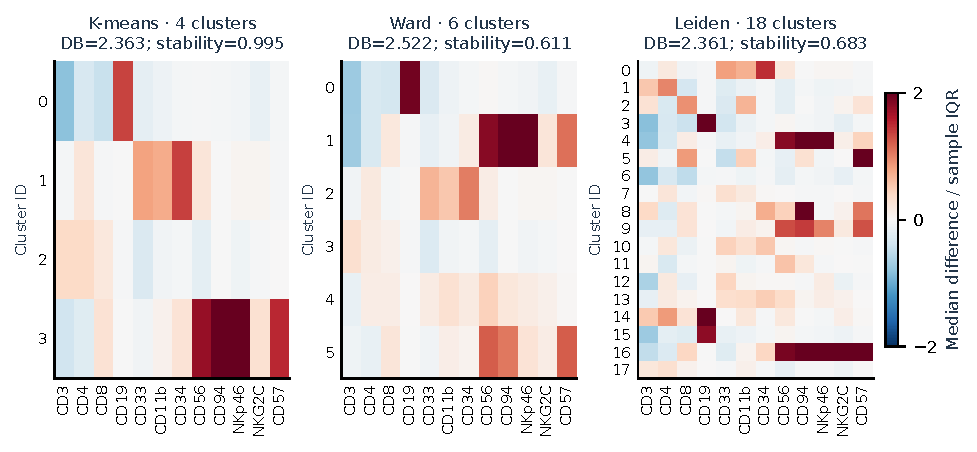
\includegraphics[width=\linewidth]{clustering.pdf}
\caption{Marker evidence for the selected k-means, Ward and Leiden solutions on 20,000 live PBMCs. Twelve markers share one relative-IQR scale with colours clipped at $\pm2$. Cluster IDs are local to each method. DB is evaluated in 37D. Stability comes from the original ten cell-subsampling repeats. Full profiles appear in \supp{S2}.}
\label{fig:clusters}
\end{figure}

\subsection{Clustering and biological interpretation}
K-means selects four broad groups with mean stability 0.995. Ward yields six groups (0.611), and Leiden 18 (0.683). The DB scores of k-means and Leiden are nearly equal (Fig.~\ref{fig:clusters}). Marker evidence is informative at several resolutions: the CD19-enriched k-means group is B-compatible, while its NKp46/CD94-enriched group is NK-associated. Ward also separates CD19-enriched and CD56/CD94/NKp46-enriched groups. Leiden resolves a strongly NKG2C/CD57-enriched group of 281 cells, illustrating the detail available at finer resolution. These descriptions concern relative marker medians, not validated cell-type labels or proof of single-cell co-expression.

The best single-linkage score is misleading biologically: it separates 19,999 cells from one event despite DB $=0.264$ and stability $=1$. Moreover, three of six Ward clusters and four of 18 Leiden clusters have stability below 0.6 even though their method averages pass. K-means is therefore the strongest reproducible coarse description here. Ward and Leiden offer subdivisions requiring further validation. This stability assessment concerns cell removal within the sampled cohort, rather than replication in new donors. No universally superior biological partition is established without reference annotations.

\subsection{Classification benchmark}
CellCNN and SVM both achieve median test AUC 0.875, compared with 0.625 for Citrus (Fig.~\ref{fig:benchmark}). CellCNN exceeds SVM in 12 splits, ties in 12 and falls below it in six. Its mean paired AUC advantage is only 0.0167. Against Citrus, the corresponding counts are 22/6/2. Median balanced accuracy is 0.625 for CellCNN/SVM and 0.500 for Citrus, showing that good rankings do not automatically produce strong thresholded decisions. Each test set supplies only eight positive--negative donor pairs, making AUC sensitive to individual rankings. Repeated splits therefore describe variation within this cohort. Complete metric distributions are in \supp{S5}.

\begin{figure}[tb]
\centering
\includegraphics[width=\linewidth]{v02/classification.pdf}
\caption{Performance on 30 shared splits of 20 donors. A shows test AUC and B shows paired AUC differences on identical splits. Boxes span Q1--Q3 with median lines and whiskers to the most extreme values within 1.5 IQR of the box. Dots are splits. Counts denote better/equal/worse performance of the first method. Overlapping splits describe variation within this cohort, not confidence intervals.}
\label{fig:benchmark}
\end{figure}

\newpage
\subsection{Model-associated cell subsets}
The common test-cell analysis reveals different selection patterns (Fig.~\ref{fig:subsets}). CellCNN, SVM and Citrus select 863, 93 and 1,583 map cells at least once, but only 84, 9 and 11 in at least half of their donor's test appearances. CellCNN has a consistent core within a broader, less stable selection, whereas Citrus marks many cells intermittently. Fifteen CellCNN reference cells are selected in every test appearance, compared with none for SVM or Citrus. Each cell counts only once per split, so recurrence reflects reproducibility of its selection rather than the number of filters or nested clusters selecting it. CellCNN/SVM profiles show stronger NKG2C enrichment (mean reference z-scores 2.862/3.004) than Citrus (0.972), alongside NK-associated markers. This is compatible with the CMV-related phenotype described by Horowitz et al.~\cite{horowitz}, but the pooled profiles can mix populations. Tracking the same cells permits comparison without aligning individual filters or clusters between splits. Different selection rules prevent interpreting cell counts alone as biological superiority.

\begin{figure}[htb]
\centering
\includegraphics[width=\linewidth]{v02/subsets.pdf}
\caption{A--C show the same 10,000 \texttt{gated\_alive} reference cells on t-SNE (perplexity 30). Colour is selections divided by the donor's 4--16 outer test appearances across 30 splits. Grey means never selected. Panel counts indicate selection at least once and in at least half of test appearances. D shows full-test-donor marker profiles on a common z-scale, averaging selected cells within nonempty visits, then visits within donors and all 20 donors equally. Empty selections remain in frequency denominators but have no marker profile. Selection rules differ by method.}
\label{fig:subsets}
\end{figure}

\clearpage
\subsection{Exploratory extension: modified CellCNN}
\label{sec:bonus}
We add diagonal quadratic terms, $\relu(b_f+w_f^Tz+q_f^Tz^{\odot2})$, to capture nonlinear marker responses without cross-marker products. The quadratic weights start at zero, so the hard-pooling variant contains the linear baseline at initialisation. We compare hard top-1\% pooling with a learnable fraction that smoothly weights sorted responses, and include a diagonal Mahalanobis/ReLU prototype variant (\supp{S4}). The latter constrains responses to neighbourhoods of learned centres and uses a different regularisation scheme. Its result is therefore not an isolated test of distance geometry. On 100 shared splits, both quadratic variants increase mean AUC by 0.1050. Soft pooling adds no further mean AUC gain. The prototype variant performs worse. These are exploratory comparisons on the same small donor cohort.

\begin{center}\small
\begin{tabular}{@{}lr@{}}\toprule
Model & Mean network AUC (100 splits)\\\midrule
CellCNN baseline & 0.8075\\
Quadratic Top-1\% & 0.9125\\
Quadratic Soft-$\alpha$ & 0.9125\\
Mahalanobis/ReLU Soft-$\alpha$ & 0.7375\\\bottomrule
\end{tabular}
\end{center}

\section{Discussion and conclusion}
The analyses answer complementary questions: embedding quality concerns geometry, clustering stability concerns reproducibility within the sampled cells, and held-out classification concerns donor prediction. None alone validates a biological cell type. Twenty donors, including related individuals, repeated overlapping splits and heuristic subset thresholds limit generalisation. Joint exploratory projections are also distinct from independent biological validation. CellCNN and SVM give similar rankings, while their cell selections differ. Citrus is weaker in this benchmark.

The benchmark compares complete implementations: CellCNN retains an inner-fold model while the baselines refit on all training donors, and their donor inputs differ in size. Performance differences therefore cannot be attributed solely to the model family. Equal cell sampling prevents large donor files from dominating the analysis, but cannot substitute for more independent donors. Future evaluation should keep related donors together and assess sensitivity to subset thresholds before comparing the resulting populations with reference annotations. Quadratic filters are a promising extension, but confirmation requires an independent donor cohort and biological assessment of the selected cells.

\begingroup
\footnotesize
\raggedright
\setlength{\bibsep}{1.5pt}
\begin{thebibliography}{10}
\bibitem{cellcnn} E.~Arvaniti and M.~Claassen. Sensitive detection of rare disease-associated cell subsets via representation learning. \emph{Nat. Commun.} 8:14825, 2017. \href{https://doi.org/10.1038/ncomms14825}{doi:10.1038/ncomms14825}.
\bibitem{horowitz} A.~Horowitz et al. Genetic and environmental determinants of human NK cell diversity revealed by mass cytometry. \emph{Sci. Transl. Med.} 5:208ra145, 2013. \href{https://doi.org/10.1126/scitranslmed.3006702}{doi:10.1126/scitranslmed.3006702}.
\bibitem{citrus} R.~V.~Bruggner et al. Automated identification of stratifying signatures in cellular subpopulations. \emph{PNAS} 111:E2770--E2777, 2014. \href{https://doi.org/10.1073/pnas.1408792111}{doi:10.1073/pnas.1408792111}.
\bibitem{tsne} L.~van der Maaten and G.~Hinton. Visualizing data using t-SNE. \emph{JMLR} 9:2579--2605, 2008. \href{https://www.jmlr.org/papers/v9/vandermaaten08a.html}{jmlr.org/papers/v9/vandermaaten08a.html}.
\bibitem{umap} L.~McInnes, J.~Healy and J.~Melville. UMAP: Uniform manifold approximation and projection for dimension reduction. \emph{arXiv:1802.03426}, 2018. \href{https://doi.org/10.48550/arXiv.1802.03426}{doi:10.48550/arXiv.1802.03426}.
\bibitem{trust} J.~Venna and S.~Kaski. Neighborhood preservation in nonlinear projection methods: an experimental study. \emph{ICANN}, pp.~485--491, 2001. \href{https://doi.org/10.1007/3-540-44668-0_68}{doi:10.1007/3-540-44668-0\_68}.
\bibitem{db} D.~L.~Davies and D.~W.~Bouldin. A cluster separation measure. \emph{IEEE TPAMI} PAMI-1:224--227, 1979. \href{https://doi.org/10.1109/TPAMI.1979.4766909}{doi:10.1109/TPAMI.1979.4766909}.
\bibitem{leiden} V.~A.~Traag, L.~Waltman and N.~J.~van Eck. From Louvain to Leiden: guaranteeing well-connected communities. \emph{Sci. Rep.} 9:5233, 2019. \href{https://doi.org/10.1038/s41598-019-41695-z}{doi:10.1038/s41598-019-41695-z}.
\bibitem{scipy} P.~Virtanen et al. SciPy 1.0: fundamental algorithms for scientific computing in Python. \emph{Nat. Methods} 17:261--272, 2020. \href{https://doi.org/10.1038/s41592-019-0686-2}{doi:10.1038/s41592-019-0686-2}.
\bibitem{sklearn} F.~Pedregosa et al. Scikit-learn: machine learning in Python. \emph{JMLR} 12:2825--2830, 2011. \href{https://www.jmlr.org/papers/v12/pedregosa11a.html}{jmlr.org/papers/v12/pedregosa11a.html}.
\end{thebibliography}
\endgroup


\end{document}
